\section{Filtros de segundo orden}
\subsection{Filtro Pasa-Bajos}
El filtro a analizar en la sección se muestra en el esquemárico \ref{ESQUEMÁTICO DE LOS FILTROS}.

\begin{figure}[H]
    \centering
    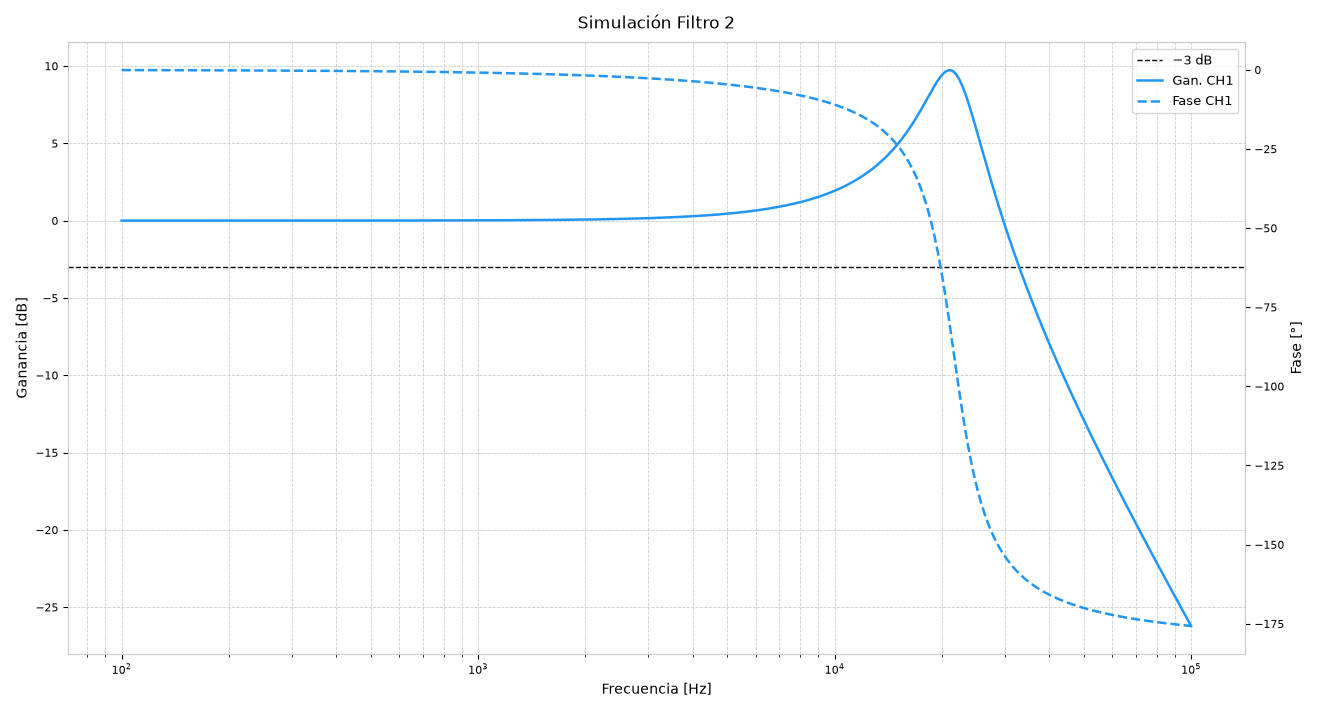
\includegraphics[width=1\textwidth]{FILTRO_2.png}
    \caption{respuesta medida del filtro pasa-bajos}
    \label{fig:Pasa_B_real}
\end{figure}

\begin{figure}[H]
    \centering
    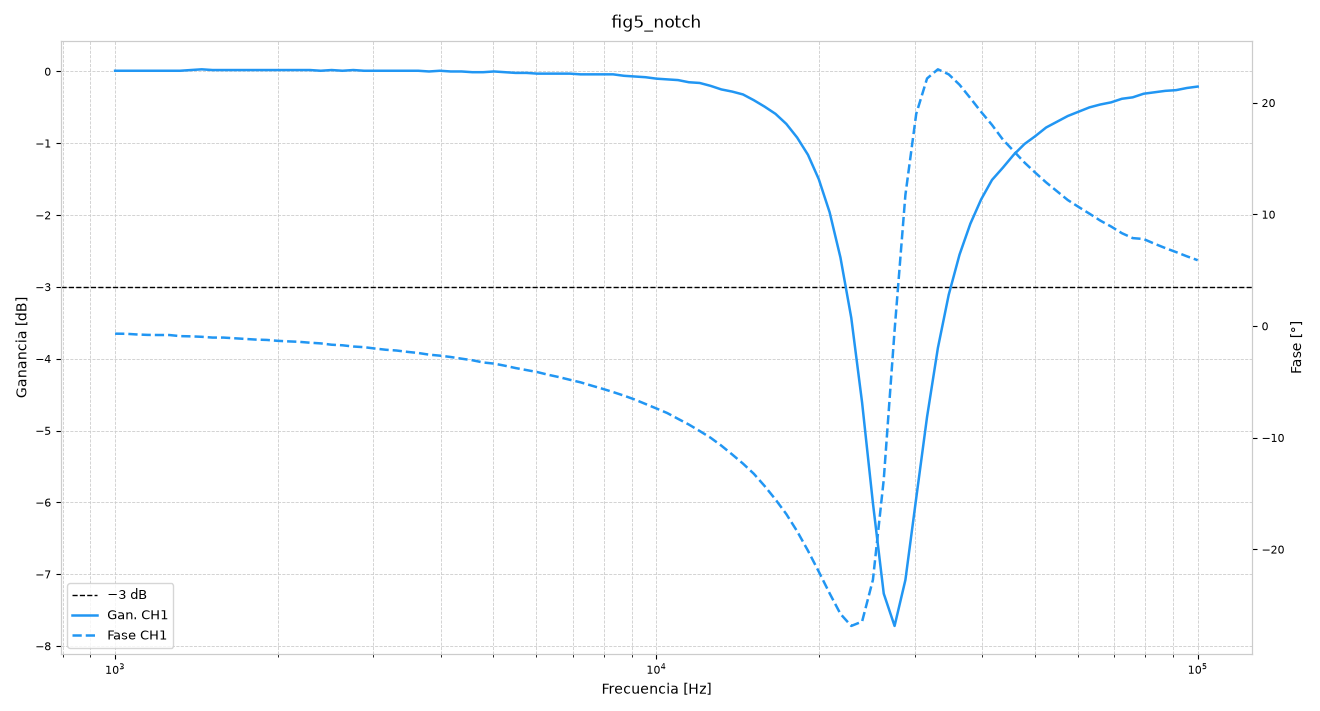
\includegraphics[width=1\textwidth]{FILTRO_2_sim.png}
    \caption{respuesta simulada del filtro pasa-bajos}
    \label{fig:Pasa_B_sim}
\end{figure}



En este caso, se presenta un filtro pasa-bajos cuya frecuencia de corte es aproximadamente $22kHz$ en la simulación y en la realidad es un poco mayor. Esta diferencia puede ser  causa de una inductancia real menor. 

Sin embargo, se percive que el filtro real posee un ancho de banda mayor al filtro simulado. Además, se observa que el sobrepico en el simulado es mayor que en el real. Consecuentemente, el factor de calidad($Q$) de este polo deberá ser menor al simulado pues $Q = \frac{\omega_0}{\Delta\omega}$ y $Q = \frac{1}{2\xi}$. Esto tiene sentido considerando que se está utilizando un inductor no comercial cuyas pérdidas se acrecentan con la frecuencia. Entonces la resistencia del circuito analizado en la realidad debería ser mayor y, pues el factor de calidad es inversamente proporcional a la resistencia, el $Q$ deberá ser menor.

\subsection{Filtro Notch}
El filtro notch es el que se muestra en la figura \ref{ESQUEMÁTICO DE LOS FILTROS}. 
Este filtro se ha medido en el laboratorio dando la siguiente respuesta:

\begin{figure}[H]
    \centering
    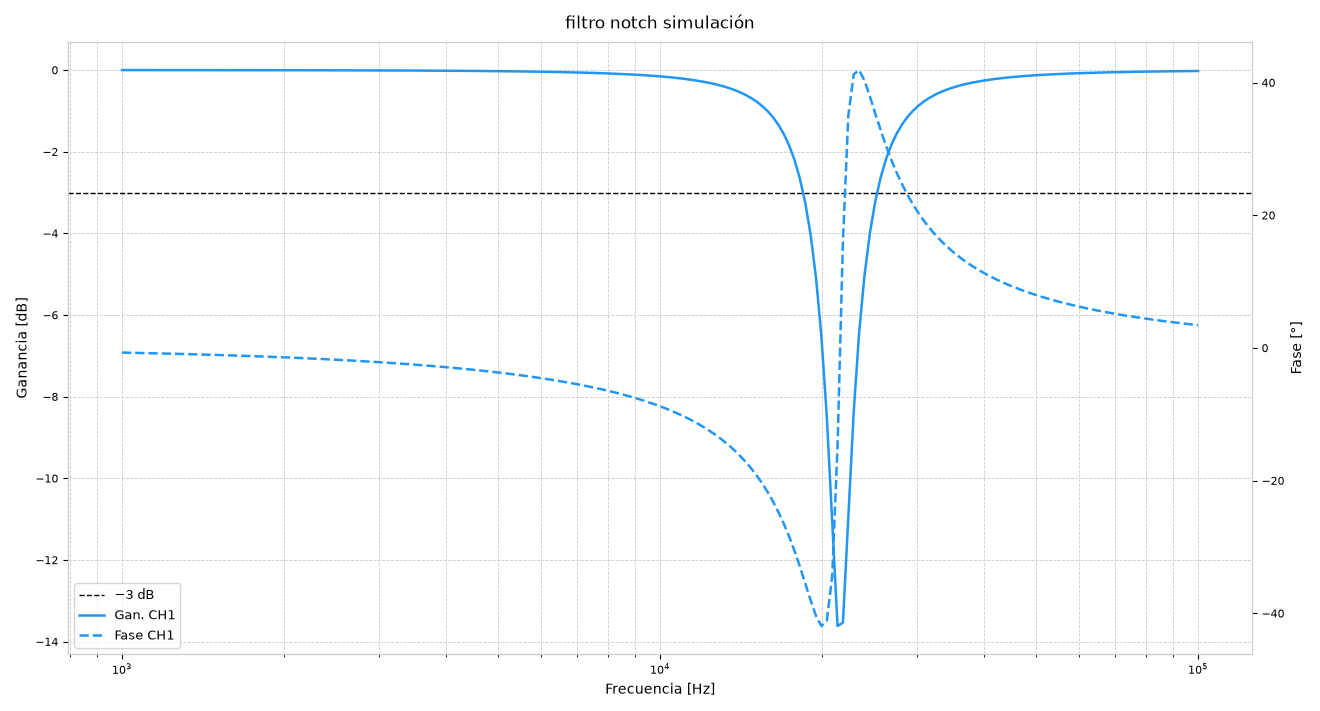
\includegraphics[width=1\textwidth]{FILTRO_5.png}
    \caption{respuesta medida del filtro notch}
    \label{fig:otch_real}
\end{figure}

\begin{figure}[H]
    \centering
    
\includegraphics[width=1\textwidth]{FILTRO_5_sim.png}
    \caption{respuesta simulada del filtro notch}
    \label{fig:notch_sim}
\end{figure}

La frecuencia  de resonancia teórica es aproximadamente $22kHz$, la misma que la del filtro pasa-bajos. La frecuencia de resonancia real tambén es un poco más alta. Se nota un comportamiento similar con el filtro anterior. El ancho de banda es mayor en el real en comparación con el simulado. En conclusión, el comportamiento se replica cambiando la salida del circuito y sin modificar los componentes. Por lo tanto, la discrepancia entre el circuito simulado y el circuito real deberá estar en las pérdidas no consideradas del inductor. 